
\begin{lead}

 信号の長さが適当な有限長であれば,その周波数解析をDFTに基づいて行い,FFTアルゴリズムを使用することができる.
%
このため,コンピュータを利用して周波数解析を容易に行うことができると考えられるが,時間信号の長さを考慮しなければならないため,実際問題として簡単なことではない.

 そこで,長い時間信号のある区間を切り出して,その切り出された信号に対して周波数解析を行う必要がある.ここでは,この信号の切り出しの方法と,切り出しの影響について説明する.


\end{lead}

%\vfill

%\begin{koumoku}
%高速フーリエ変換(FFT)\\
%複素指数関数\\
%位相回転因子\\
%時間間引き\\
%乗算回数
%\end{koumoku}

%\clearpage

\chapter{窓関数}
\label{chapter:window}

\section{窓関数}

前章で学んだように,信号の長さが適当な有限長であれば,その周波数解析をDFTに基づいて行うことができるので,FFTアルゴリズムを使用できる可能性が高い.このため,コンピュータを利用して周波数解析を容易に行うことができる.

しかしながら,\index{おんせいしんごう@音声信号}音声信号に代表されるように,ディジタル信号において取り扱われる信号の多くは非常に長く,データ量が膨大である.このような信号の全体を一度にコンピュータを用いて処理することは一般的にはできない.
%
なぜなら,コンピュータの能力が有限であることから,一度に処理できるデータ量には限界があることと,信号全体を取り込むのに要する膨大な遅延時間が許容されないという理由があるためである.

そこで,長い時間信号のある区間を切り出して,それに対して周波数解析を行う必要がある.そのために必要となる関数が\index{まどかんすう@窓関数}窓関数である.ここでは,信号の切り出しの方法と,切り出しの影響について説明する.

\subsection{窓関数による信号の切り出し}

図\ref{fig:window-1}に示す信号$x(n)$の有限区間を切り出す方法を考える.対象となる信号$x(n)$に有限な範囲外で零値をとる$w(n)$を乗算することによって,信号を取り出すものとする.すなわち,
\begin{equation}
x_w(n)=x(n)w(n)
\end{equation}
と切り出された信号$x_w(n)$を解析する.切り出しに用いた有限の信号$w(n)$を窓関数(window function)という.

\begin{figure}[H]
\begin{center}
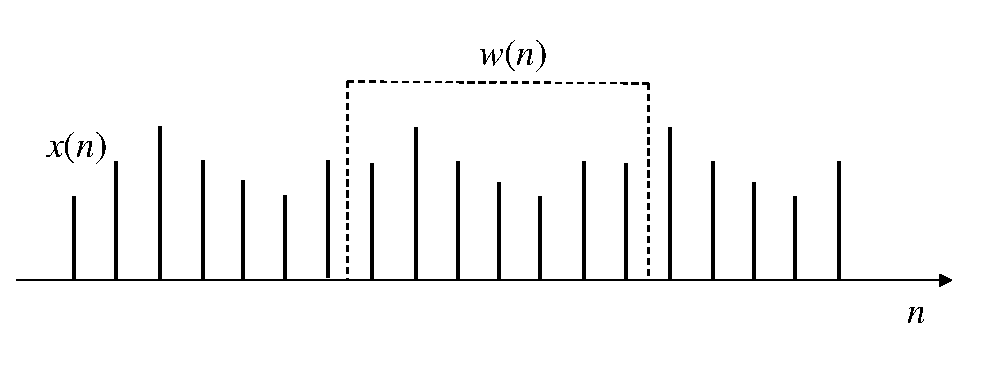
\includegraphics[width=.45\textwidth]{fig/window-1.eps}

(a) 実際の信号$x(n)$

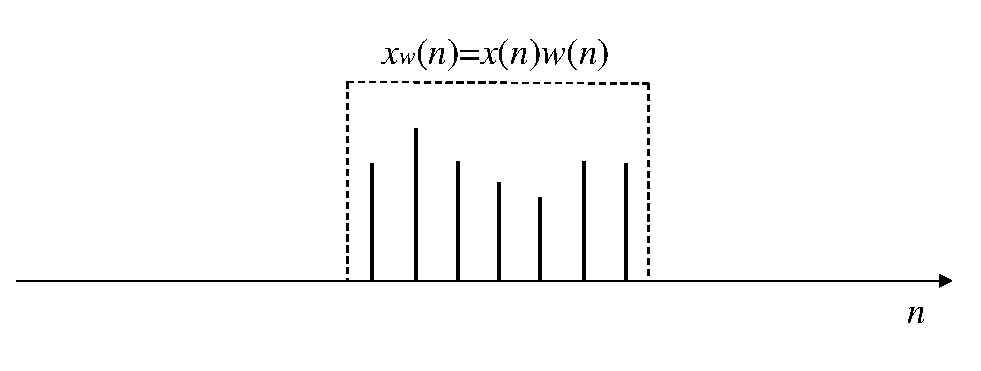
\includegraphics[width=.45\textwidth]{fig/window-2.eps}

(b) 窓関数$w(n)$で切り出された信号$w(n)x(n)$
\end{center}\vskip.5\baselineskip
\caption{窓関数$w(n)$による信号の切り出し}
\label{fig:window-1}
\end{figure}



窓関数$w(n)$の長さ(零値以外の範囲)を適当に選べば,$x_w(n)$の長さを自由に選択することができて,コンピュータによってそれを解析することは容易である.しかし,$x_w(n)$の周波数スペクトルは,$x(n)$の周波数スペクトルとは異なってしまう.このため,信号の切り出しによって周波数スペクトルの受ける影響について注意を払う必要がある.

\subsection{切り出しの影響}

例として,図\ref{fig:fft-sinwave}の\index{せいげんはしんごう@正弦波信号}正弦波信号の場合について説明する.この信号は,$F=4$Hzの正弦波信号を32Hzの\index{さんぷりんぐしゅうはすう@サンプリング周波数}サンプリング周波数$F_S=1/T_s$でサンプリングした式である.これを式で表すと,

\begin{eqnarray}
x(n)&=& \cos (\omega_0 n) \nonumber \\
 &=&\frac{e^{-j\omega_0 n}+e^{-j\omega_0 n}}{2}
\label{eqn:fft-sinwave-2}
\end{eqnarray}\vskip.3\baselineskip

\noindent である.ここで,$\omega_0 = \Omega T_s = 2\pi F/F_s = \pi/4$である.

\begin{figure}[H]
\begin{center}
\begin{minipage}{.38\textwidth}
\begin{center}
%\includegraphics[width=8cm]{fig/fft-sinwave-1.eps}
\includegraphics[width=.98\textwidth]{fig/zu-7-9-a.eps}

(a)
\end{center}
\end{minipage}
\begin{minipage}{.38\textwidth}
\begin{center}
%\includegraphics[width=8cm]{fig/fft-sinwave-1.eps}
\includegraphics[width=.98\textwidth]{fig/zu-7-9-b.eps}

(b)
\end{center}
\end{minipage}
\end{center}\vskip.5\baselineskip
\caption{正弦波信号}
\label{fig:fft-sinwave}
\end{figure}

この信号は\index{しゅうきてき@周期的}周期的な\index{りさんじかんしんごう@離散時間信号}離散時間信号であるため,解析は離散時間フーリエ級数に基づいて行われる.次式のフーリエ係数$X_N(k)$
\begin{equation}
X_N(k) = \sum_{n=0}^{N-1}x_N(n) e^{-j2\pi nk / N}
\label{eqn:fft-sinwave-21}
\end{equation}
を用いると,式(\ref{eqn:fft-sinwave-2})は
\begin{equation}
x(n) = \frac{1}{N} (X_N(-1)e^{-j\omega_0 n} +X_N(1)e^{j\omega_0 n})
\label{eqn:fft-sinwave-3}
\end{equation}
と書き直すことができる.ここで,$N$は1周期の点数で$N=8$であり,$X(-1)=X(1)=4$となる.したがって,図\ref{fig:fft-sinwave}(b)の\index{しゅうはすうすぺくとる@周波数スペクトル}周波数スペクトルが対応する.

次に,図\ref{fig:fft-sinwave-2}に示すように,窓関数$w(n)$を$X(n)$に乗じて信号を切り出し,この$x_w(n)=x(n)w(n)$と$x(n)$との周波数スペクトルのちがいを見ることにする.ちがいは,信号を切り出した影響と考えることができ,図\ref{fig:fft-sinwave-2}(b)に示すように図\ref{fig:fft-sinwave}(b)とは異なるものとなった.

\begin{figure}[H]
\begin{center}
\begin{minipage}{.38\textwidth}
\begin{center}
%\includegraphics[width=8cm]{fig/fft-sinwave-1.eps}
\includegraphics[width=.9\textwidth]{fig/zu-7-10-a.eps}

(a)
\end{center}
\end{minipage}
\begin{minipage}{.38\textwidth}
\begin{center}
%\includegraphics[width=8cm]{fig/fft-sinwave-1.eps}
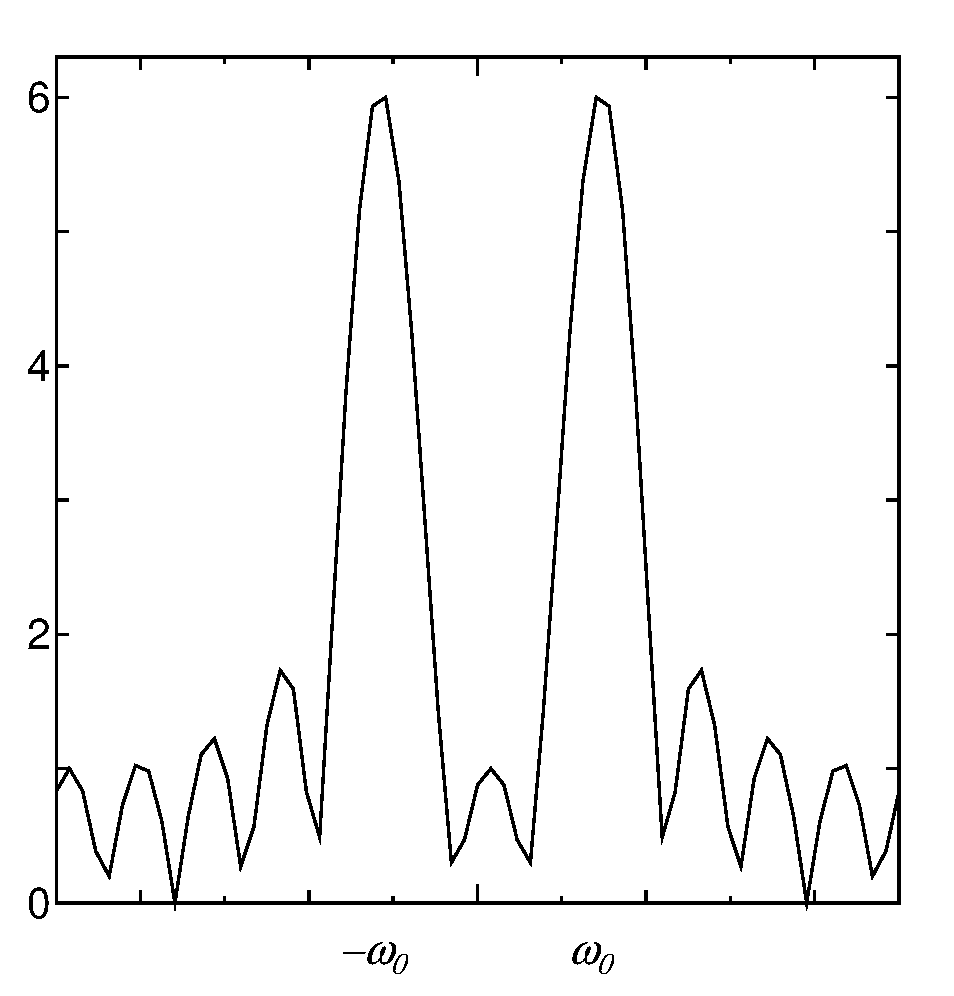
\includegraphics[width=.9\textwidth]{fig/zu-7-10-b.eps}

(b)
\end{center}
\end{minipage}\vskip.5\baselineskip
\end{center}
\caption{正弦波信号を窓長12で切り出した場合}
\label{fig:fft-sinwave-2}
\end{figure}


その理由を説明する.式(\ref{eqn:fft-sinwave-21})より,$x_w=x(n)w(n)$は,
\begin{equation}
x_w(n)=\frac{1}{2}w(n)e^{-j\omega_0 n)}+\frac{1}{2}w(n)e^{j\omega_0 n)}
\end{equation}
である.この$x_w(n)$の離散フーリエ変換$X_w(e^{j\omega})$は周波数シフトの性質から,
\begin{equation}
X_w(e^{j\omega})=\frac{1}{2}W(e^{j(\omega+\omega_0)})+\frac{1}{2}W(e^{j(\omega-\omega_0)})
\end{equation}
と表現される.ただし,$W(e^{j\omega})$は$w(n)$の離散フーリエ変換である.このように,窓関数$w(n)$の離散フーリエ変換$W(e^{j\omega})$が周波数シフトをした形で,信号の切り出しの影響が現れることがわかる.

\subsection{メインローブとサイドローブ}

先述における切り出しの影響をさらに詳しく見るために,窓関数の周波数スペクトル$W(e^{j\omega})$に着目する.図\ref{fig:main-side-lobe}(a)は,図\ref{fig:fft-sinwave-2}に示した例で用いた窓関数とそのスペクトルである.ここで$\omega=0$を中心に存在するスペクトルの主部をメインローブ(main lobe),\index{めいんろーう゛@メインローブ}メインローブ以外のスペクトルを\index{さいどろーぶ@サイドローブ}サイドローブ(side lobe)と呼ぶ.

図\ref{fig:fft-sinwave-2}と図\ref{fig:fft-sinwave}との比較から,\index{きりだしのえいきょう@切り出しの影響}切り出しの影響を抑えるためには,窓関数に対して以下の条件を満たすことが望まれている.

\begin{itemize}
\item メインローブが急峻であること
\item サイドローブが小さいこと
\end{itemize}
%
しかし,ある限られた長さの窓関数であれば,両者を同時に望むことはできず,お互いにトレードオフの関係である.

また,窓関数の長さに自由度があるときには,メインローブを急峻にするために,許容できる最大の長さを使用する必要がある.
たとえば,図\ref{fig:main-side-lobe}(b)のように窓関数の長さを2倍にすると,スペクトルは周波数上で半分に縮小し,結果としてメインローブは急峻となる.
メインローブの急峻さは近接した周波数スペクトルを持つ信号を解析する場合に,サイドローブは大きさの異なるスペクトルを解析する場合に重要である.

\begin{figure}[H]
\begin{center}
\begin{minipage}{.38\textwidth}
\begin{center}
%\includegraphics[width=8cm]{fig/fft-sinwave-1.eps}
\includegraphics[width=.98\textwidth]{fig/zu-7-11-a-1.eps}

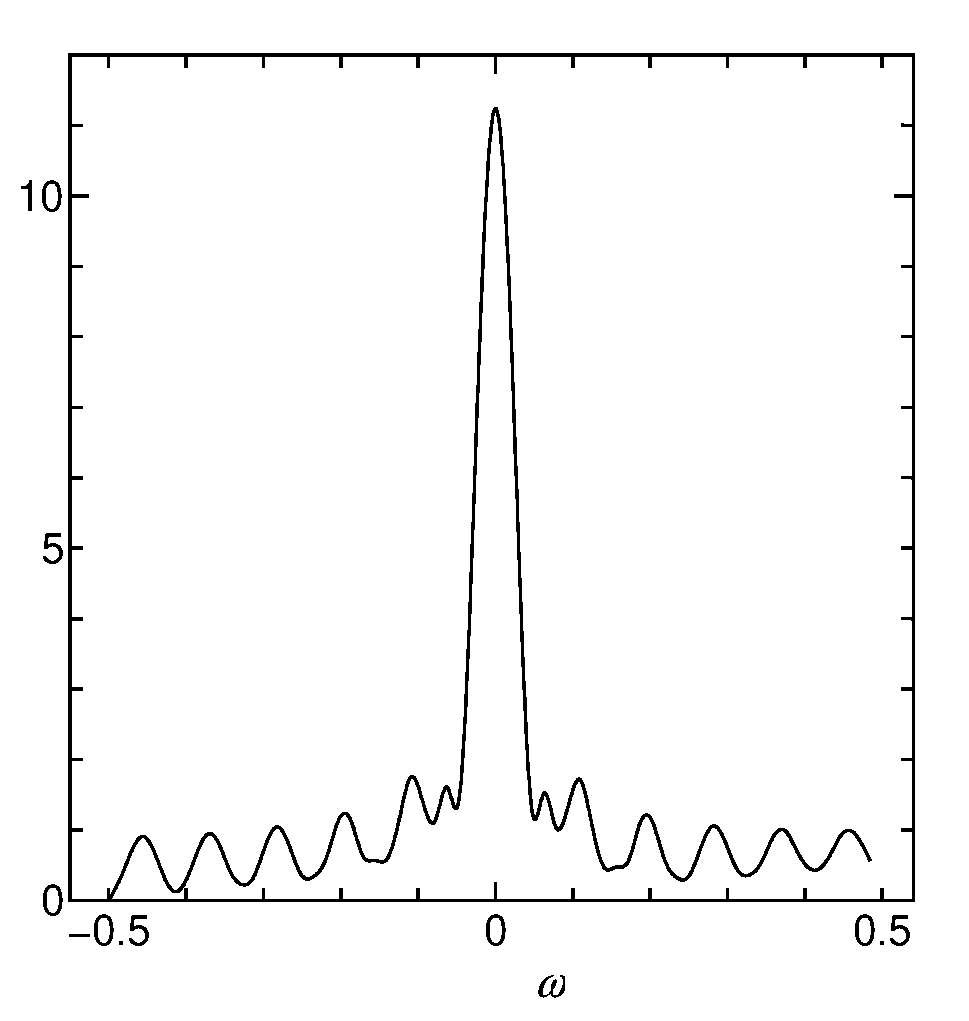
\includegraphics[width=.98\textwidth]{fig/zu-7-11-a-2.eps}

(a) 窓幅12
\end{center}
\end{minipage}
\begin{minipage}{.38\textwidth}
\begin{center}
%\includegraphics[width=8cm]{fig/fft-sinwave-1.eps}
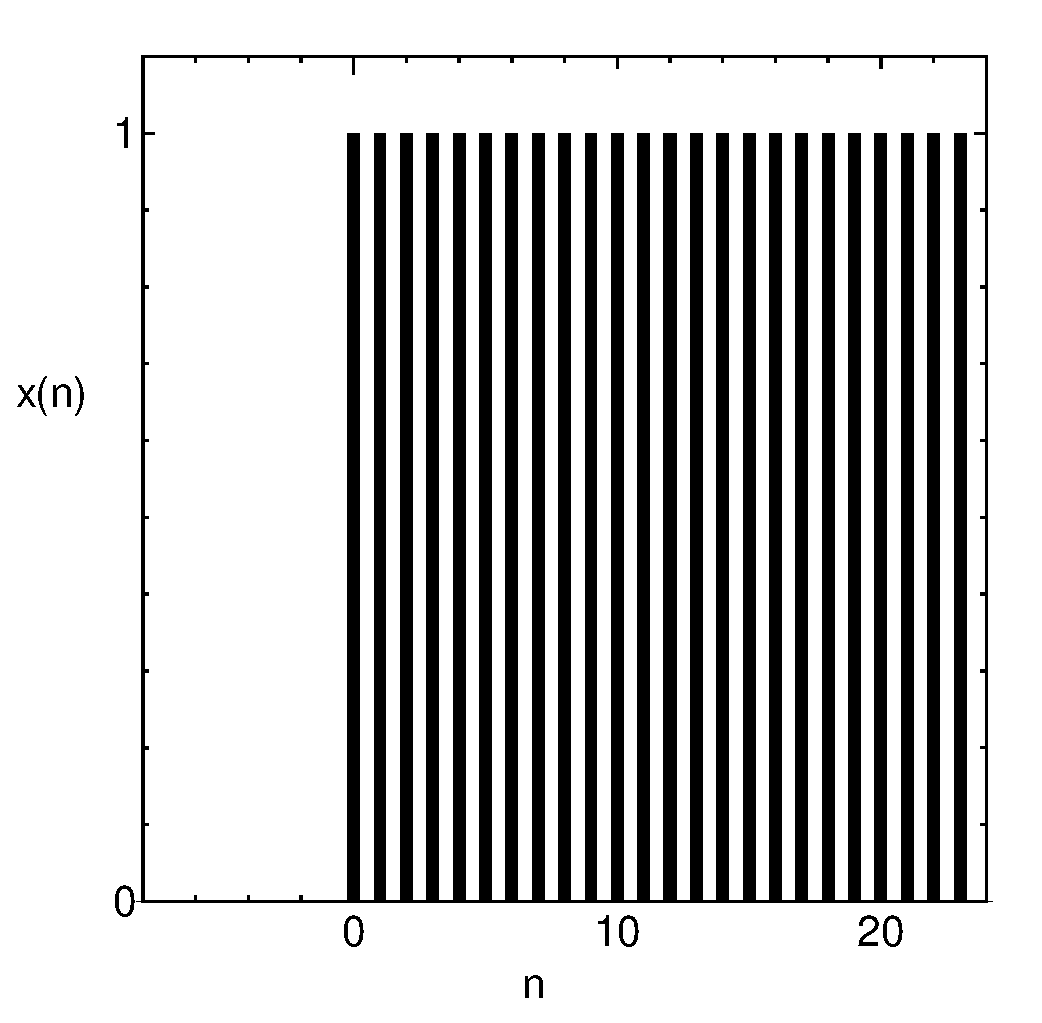
\includegraphics[width=.98\textwidth]{fig/zu-7-11-b-1.eps}

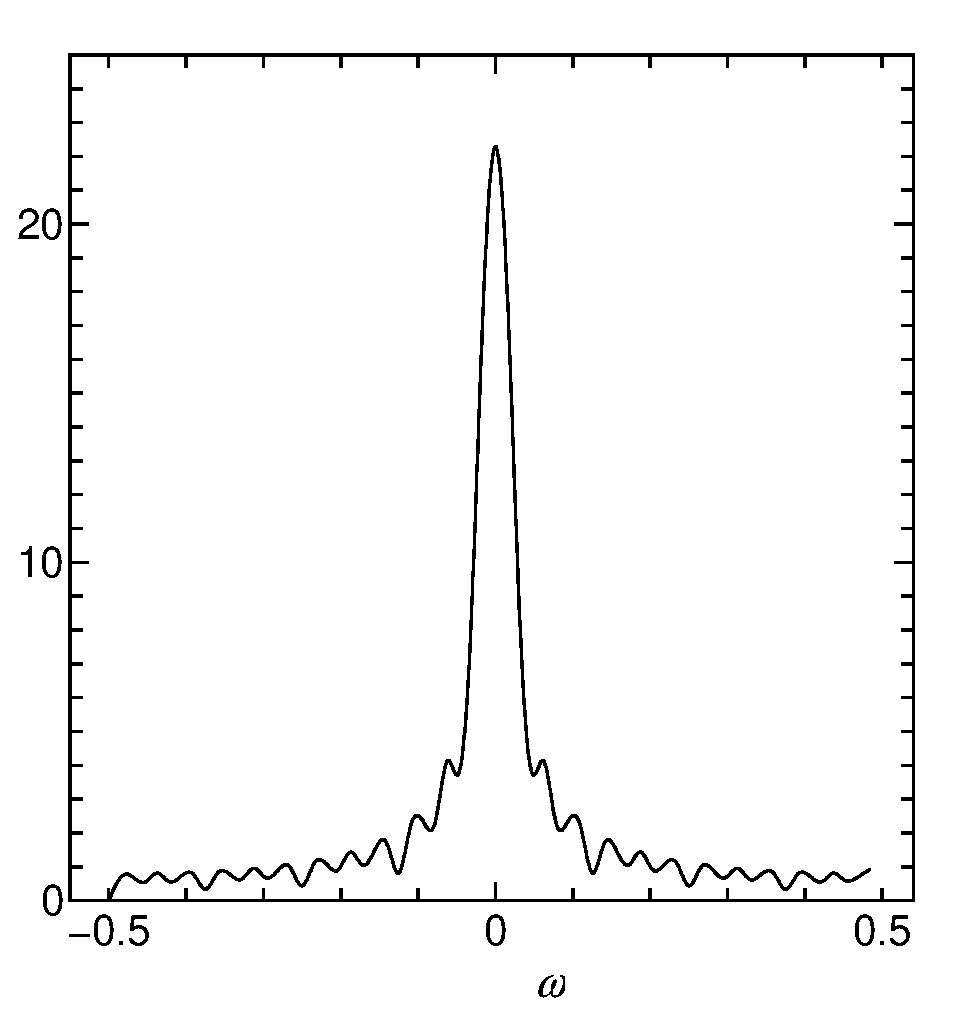
\includegraphics[width=.98\textwidth]{fig/zu-7-11-b-2.eps}

(b) 窓幅24
\end{center}
\end{minipage}
\end{center}\vskip.5\baselineskip
\caption{窓関数$w(n)$と周波数スペクトル}
\label{fig:main-side-lobe}
\end{figure}


\section{代表的な窓関数}

窓関数のメインローブとサイドローブが,\index{しゅうはすうかいせき@周波数解析}周波数解析において重要な役割を果たすことが示された.メインローブとサイドローブのちがいにより,種々の窓関数が知られている.ここでは,代表的な窓関数について述べる.


\subsection{方形窓(rectangular window)}

図\ref{fig:houkei-mado}に長さ$M=15$の場合の時間波形$w(n)$とその周波数スペクトル$W(e^{j\omega})$を示す.\index{ほうけいまど@方形窓}方形窓は次式で与えられる.
\begin{equation}
w(n)= \left \{
\begin{array}{ll}
1 & (0 \leq n \leq M-1) \\
0 & その他
\end{array}
\right .
\end{equation}
ただし,周波数スペクトルは$20\log_{10} | W (e^{\textrm{j}\omega})|$なる常用対数を計算したものを用いた.この場合の単位はdB(デジベル)となる.

この窓関数は信号のひずみが少なく,基本的で単純な窓である.ただし,後述のような他の窓関数と比較すると,サイドローブの最大値は大きくなってしまうことがわかる.


\begin{figure}[H]
\begin{center}
\begin{minipage}{.38\textwidth}
\begin{center}
%\includegraphics[width=8cm]{fig/houkei-mado.eps}
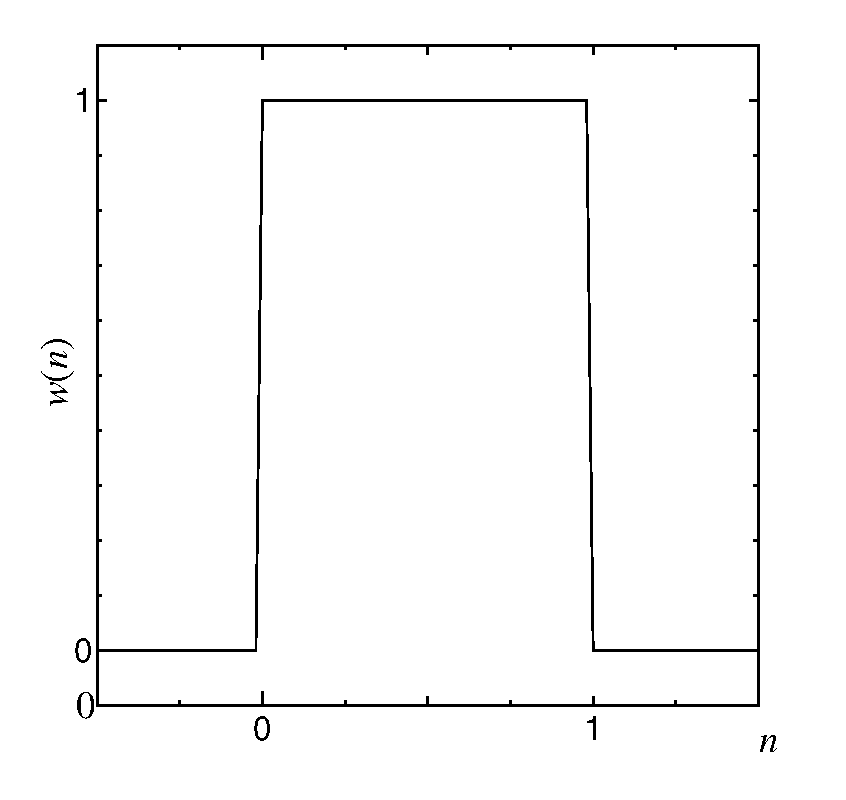
\includegraphics[width=.98\textwidth]{fig/houkei-mado-a.eps}

(a)
\end{center}
\end{minipage}
\begin{minipage}{.38\textwidth}
\begin{center}
%\includegraphics[width=8cm]{fig/haning-mado.eps}
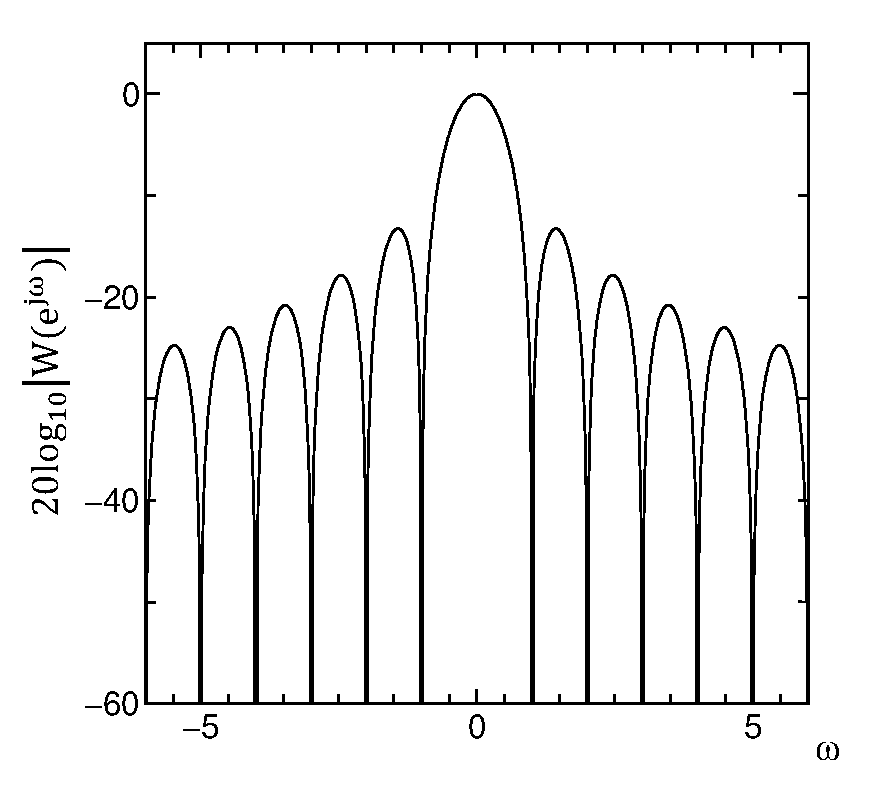
\includegraphics[width=.98\textwidth]{fig/houkei-mado-b.eps}

(b)
\end{center}
\end{minipage}
\end{center}\vskip.5\baselineskip
\caption{方形窓}
\label{fig:houkei-mado}
\end{figure}

\subsection{ハニング窓(Hanning window)}

図\ref{fig:hanning-mado}に長さ$M=15$の場合の時間波形$w(n)$とその周波数スペクトル$W(e^{j\omega})$を示す.\index{はにんぐまど@ハニング窓}ハニング窓については次式で与えられる.
\begin{equation}
w(n)= \frac{1}{2} \left \{ 1- \cos \frac{2\pi n}{M}\right \}
\end{equation}

この窓関数は,方形窓と比較するとメインローブは広いものの,サイドローブは急速に小さくなることがわかる.


\begin{figure}[H]
\begin{center}
\begin{minipage}{.38\textwidth}
\begin{center}
%\includegraphics[width=8cm]{fig/haning-mado.eps}
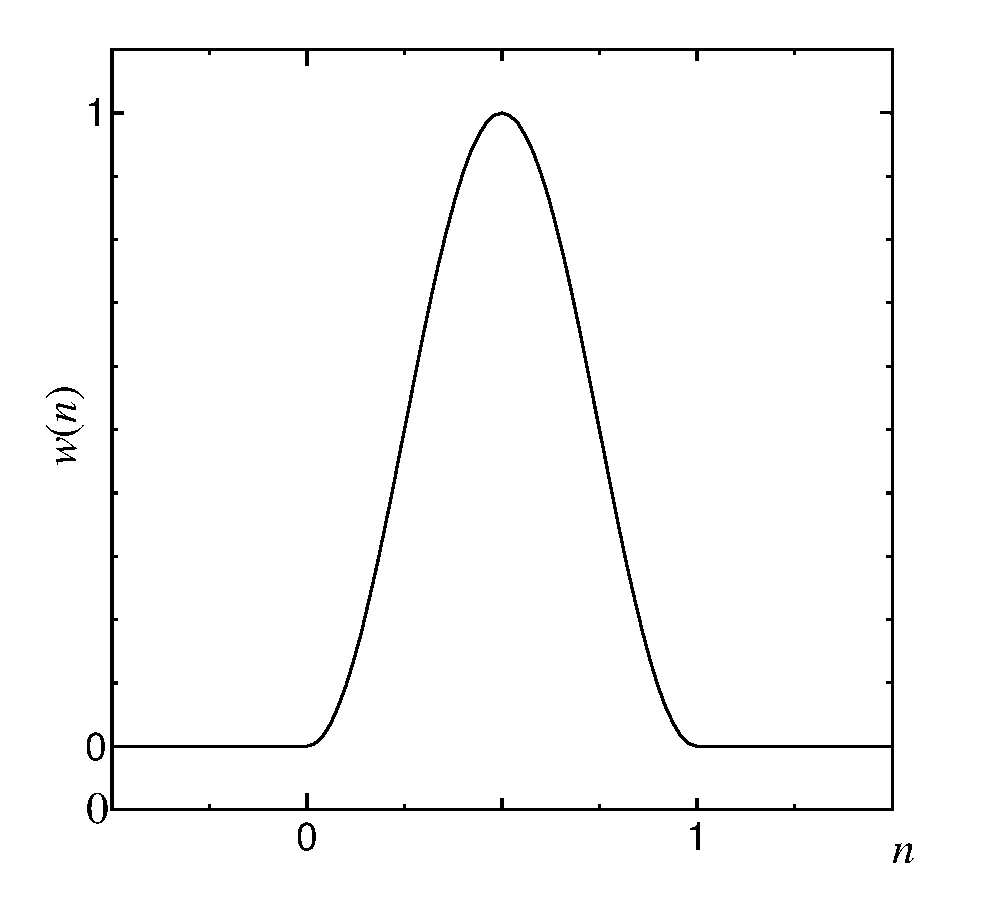
\includegraphics[width=.98\textwidth]{fig/haning-mado-a.eps}

(a)
\end{center}
\end{minipage}
\begin{minipage}{.38\textwidth}
\begin{center}
%\includegraphics[width=8cm]{fig/haning-mado.eps}
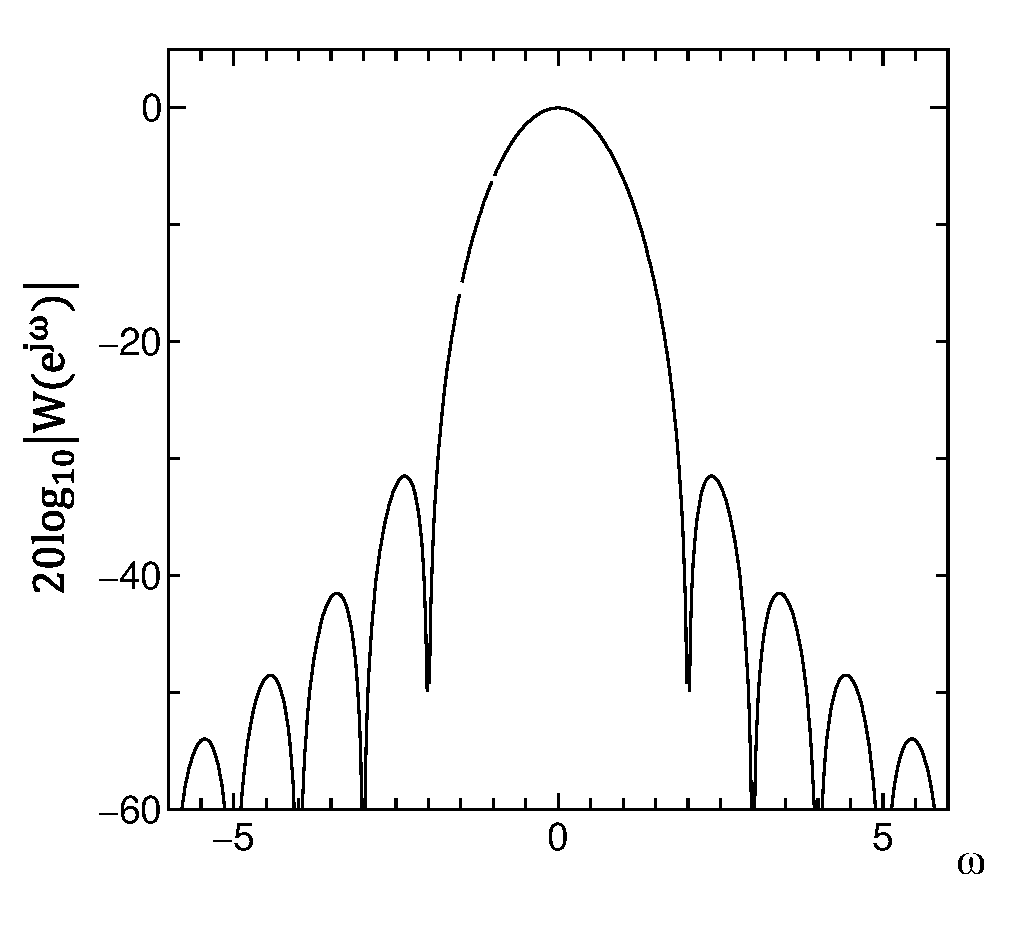
\includegraphics[width=.98\textwidth]{fig/haning-mado-b.eps}

(b)
\end{center}
\end{minipage}
%\includegraphics[width=8cm]{fig/haning-mado.eps}
\end{center}\vskip.5\baselineskip
\caption{ハニング窓}
\label{fig:hanning-mado}
\end{figure}

\subsection{ハミング窓(Hamming window)}

図\ref{fig:hamming-mado}に長さ$M=15$の場合の時間波形$w(n)$とその周波数スペクトル$W(e^{j\omega})$を示す.\index{はみんぐまど@ハミング窓}ハミング窓については次式で与えられる.
\begin{equation}
w(n)= \frac{25}{46} - \left ( 1-\frac{25}{46} \right ) \cos \frac{2\pi n}{M}
\end{equation}
この窓関数は,方形窓と比較すると,メインローブはハニング窓とほぼ同じであるが,サイドローブはメインローブ近傍の値が小さいことがわかる.


\begin{figure}[H]
\begin{center}
\begin{minipage}{.38\textwidth}
\begin{center}
%\includegraphics[width=8cm]{fig/humming-mado.eps}
\includegraphics[width=.98\textwidth]{fig/humming-mado-a.eps}

(a)
\end{center}
\end{minipage}
\begin{minipage}{.38\textwidth}
\begin{center}
%\includegraphics[width=8cm]{fig/humming-mado.eps}
\includegraphics[width=.98\textwidth]{fig/humming-mado-b.eps}

(b)
\end{center}
\end{minipage}
\end{center}\vskip.5\baselineskip
\caption{ハミング窓}
\label{fig:hamming-mado}
\end{figure}

\vspace{-\baselineskip}
\section*{演習問題}

\subsection*{問題\ref{chapter:window}.1}

図\ref{fig:win-14}に示す信号は,2Hz, 3.8Hz, および4Hzの正弦波信号
\begin{equation}
x(t)=\cos (8\pi t)+0,5 \cos (7.6\pi t)+ 0.025 \cos (4\pi t)
\end{equation}
を$F_s=16$Hzでサンプリングしたものである.窓長32と64点の窓関数を用いて,周波数スペクトルを求めよ(コンピュータを用いた計算をお勧めする).

\begin{figure}[H]
\begin{center}
\begin{minipage}{.4\textwidth}
\begin{center}
%\includegraphics[width=.98\textwidth]{fig/fig-5-14.eps}
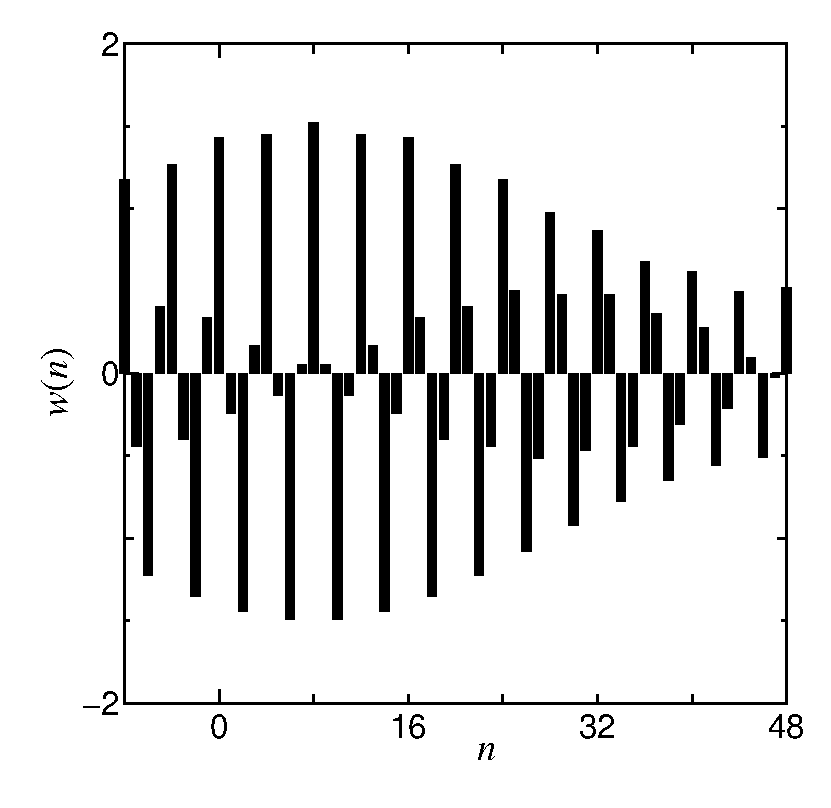
\includegraphics[width=.98\textwidth]{fig/zu-5-14-a.eps}

%(a) 信号波形
\end{center}
\end{minipage}
%\begin{minipage}{5.2cm}
%\begin{center}
%\includegraphics[width=8cm]{fig/fig-5-14.eps}
%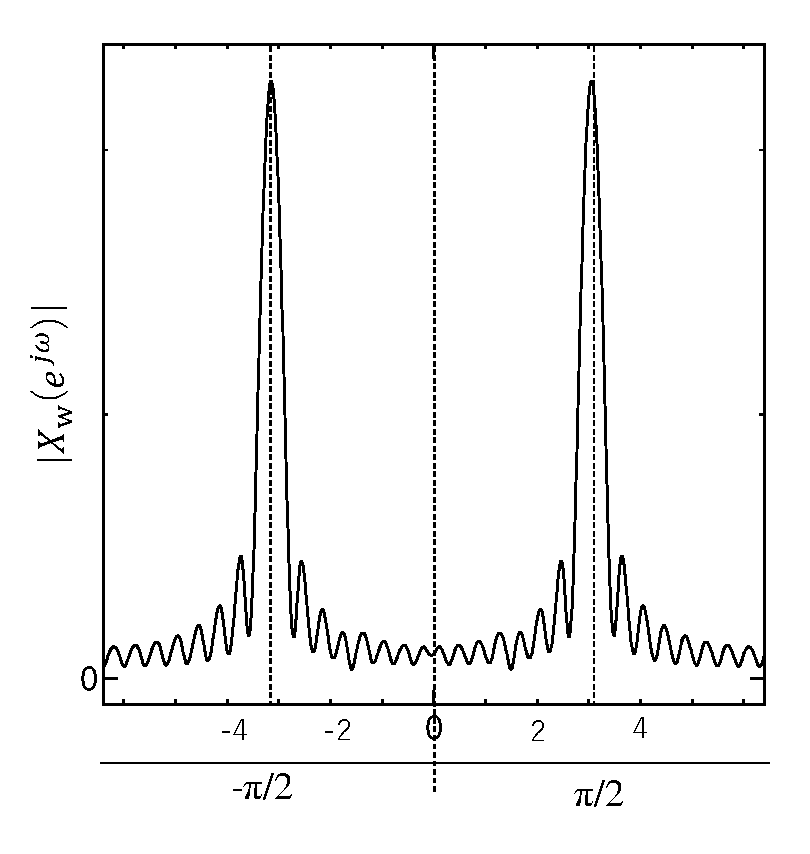
\includegraphics[width=5cm]{fig/zu-5-14-b.eps}

%(b) $M=32$のときのスペクトル
%\end{center}
%\end{minipage}
%\begin{minipage}{5.2cm}
%\begin{center}
%\includegraphics[width=8cm]{fig/fig-5-14.eps}
%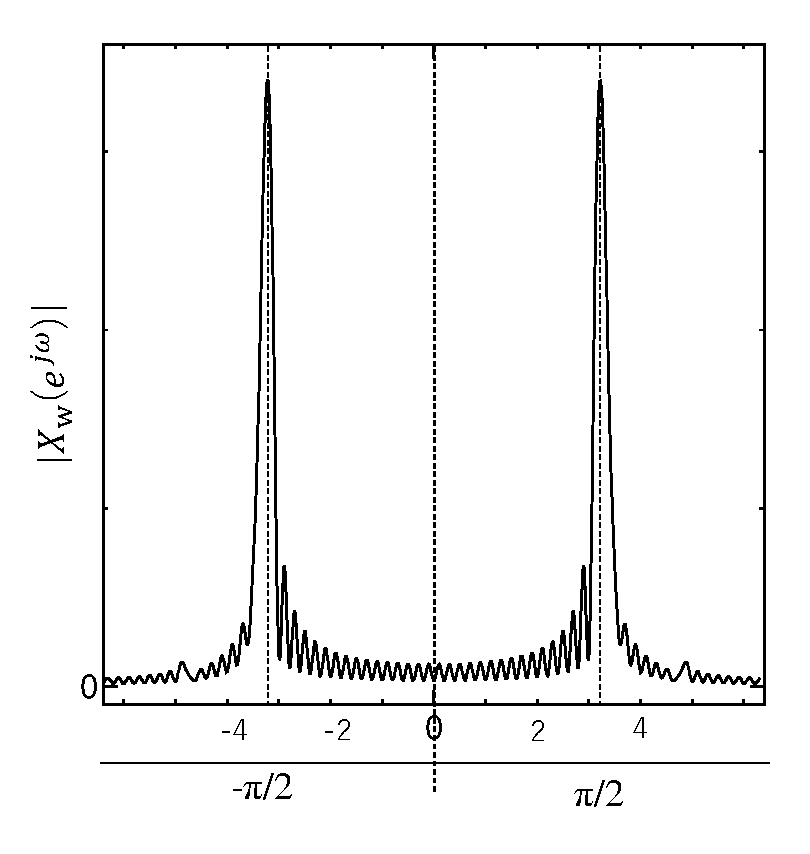
\includegraphics[width=5cm]{fig/zu-5-14-c.eps}

%(c)  $M=64$のときのスペクトル
%\end{center}
%\end{minipage}
\end{center}\vskip.5\baselineskip
\caption{問題\ref{chapter:window}.1の信号波形}
\label{fig:win-14}
\end{figure}





